\documentclass[hyperref]{article}
%MS%%%%%%%%%%%%%%%%%%%% Article Format %%%%%%%%%%%%%%%%%
%+++++++++++++++++++++ Usepackage +++++++++++++++%%
\usepackage{graphicx} %% Package for Figure
\usepackage{float} %% Package for Float
\usepackage{amssymb}
\usepackage{amsmath}
\usepackage{mathtools}
\usepackage[thmmarks,amsmath]{ntheorem} %% If amsmath is applied, then amsma is necessary
\usepackage{bm} %% Bold Mathematical Symbols
\usepackage[colorlinks,linkcolor=cyan,citecolor=cyan]{hyperref}
\usepackage{extarrows}
\usepackage[hang,flushmargin]{footmisc} %% Let the footnote not indentation
\usepackage[square,comma,sort&compress,numbers]{natbib} %% Sort of References
\usepackage{mathrsfs} %% Swash letter
\usepackage[font=footnotesize,skip=0pt,textfont=rm,labelfont=rm]{caption,subcaption} 
%% Format of Caption for Tab. and Fig.
\usepackage{booktabs} %% tables with three lines
\usepackage{tocloft}
\usepackage{graphicx}

%\usepackage{algorithm}  
%%\usepackage{algorithmicx}  
%\usepackage{algorithmic}
\usepackage[linesnumbered,boxed,commentsnumbered,ruled]{algorithm2e}

%+++++++++++++++ Proof etc. +++++++++++++++++++++++++%%
{%% Environment of Proof
	\theoremstyle{nonumberplain}
	\theoremheaderfont{\bfseries}
	\theorembodyfont{\normalfont}
	\theoremsymbol{\mbox{$\Box$}}
	\newtheorem{proof}{Proof}
}

\usepackage{theorem}
\newtheorem{theorem}{Theorem}[section]
\newtheorem{lemma}{Lemma}[section]
\newtheorem{definition}{Definition}[section]
\newtheorem{assumption}{Assumption}[section]
\newtheorem{example}{Example}[section]
\newtheorem{corollary}{Corollary}[section]
{%% Environment of Remark
	\theoremheaderfont{\bfseries}
	\theorembodyfont{\normalfont}
	\newtheorem{remark}{Remark}[section]
}
\usepackage{abstract}
\renewcommand{\abstractnamefont}{\Large\bfseries}
%\numberwithin{equation}{section} %% Number of Equation
%++++++++++++++++++++++++++++++++ Page format ++++++++++++++++++++++++++%%
\graphicspath{{figure/}}                                 %% Path of Figures
\usepackage[a4paper]{geometry}                           %% Paper size
\geometry{left=2.5cm,right=2.5cm,top=2.5cm,bottom=2.5cm} %% Margin
\linespread{1.2}      
\usepackage{cite}

% matlab code package
\usepackage{appendix}
\usepackage{listings}%插入代码
\usepackage{color}
\lstset{%代码格式的配置
	extendedchars=false,            % Shutdown no-ASCII compatible
	language=Matlab,                % !!!选择代码的语言
	basicstyle=\footnotesize\tt,    % the size of the fonts that are used for the code
	tabsize=3,                            % sets default tabsize to 3 spaces
	numbers=left,                   % where to put the line-numbers
	numberstyle=\tiny,              % the size of the fonts that are used for the line-numbers
	stepnumber=1,                   % the step between two line-numbers. If it's 1 each line
	% will be numbered
	numbersep=5pt,                  % how far the line-numbers are from the code   %
	keywordstyle=\color[rgb]{0,0,1},                % keywords
	commentstyle=\color[rgb]{0.133,0.545,0.133},    % comments
	stringstyle=\color[rgb]{0.627,0.126,0.941},      % strings
	backgroundcolor=\color{white}, % choose the background color. You must add \usepackage{color}
	showspaces=false,               % show spaces adding particular underscores
	showstringspaces=false,         % underline spaces within strings
	showtabs=false,                 % show tabs within strings adding particular underscores
	frame=single,                   % adds a frame around the code
	captionpos=b,                   % sets the caption-position to bottom
	breaklines=true,                % sets automatic line breaking
	breakatwhitespace=false,        % sets if automatic breaks should only happen at whitespace
	title=\lstname,                 % show the filename of files included with \lstinputlisting;
	% also try caption instead of title
	mathescape=true,escapechar=?    % escape to latex with ?..?
	escapeinside={\%*}{*)},         % if you want to add a comment within your code
	%columns=fixed,                  % nice spacing
	%morestring=[m]',                % strings
	%morekeywords={%,...},%          % if you want to add more keywords to the set
	%    break,case,catch,continue,elseif,else,end,for,function,global,%
	%    if,otherwise,persistent,return,switch,try,while,...},%
}
\usepackage{enumitem}
% \setlength{\parskip}{0.4em}
\usepackage{diagbox}

                                   %% Line Spread
%MS%%%%%%%%%%%%%%%%%%%%%%%%%%%% End Format %%%%%%%%%%%%%%%%%%%%%%%%%%%%%%%%%%

%MS%%%%%%%%%%%%%%%%%%%%%%%%%%%%%%%%%%%%%%%%%%%
%MS                                         %%
%MS        The Main Body begins here        %%
%MS                                         %%
%MS%%%%%%%%%%%%%%%%%%%%%%%%%%%%%%%%%%%%%%%%%%%

%MS++++++++++++++++++++++++++++++ Title +++++++++++++++++++
\title{ME5413 Autonomous Mobile Robotics: \\ Homework 3}
\author{\textup{Chen Yihui \ \ \ A0263115N \\ Wang Renjie \ A0263387U }}
\begin{document}
	\begin{titlepage}
		\center
		\newcommand{\HRule}{\rule{\linewidth}{0.5mm}}
		
\includegraphics[width=8cm]{logo.png}\\[1cm] 
		\quad\\[2cm]
		\textsl{\Large National University of Singapore}\\[0.5cm] 
		\textsl{\large College of Design and Engineering}\\[0.5cm]
		\makeatletter
		\HRule \\[0.4cm]
		{ \huge \bfseries \@title}\\[0.4cm] 
		\HRule \\[2cm]
		\begin{minipage}{0.4\textwidth}
			\begin{flushleft} \large
				\emph{Group 9:}\\
				\@author 
			\end{flushleft}
		\end{minipage}
		~
		\begin{minipage}{0.4\textwidth}
			\begin{flushright} \large
				\emph{Supervisor:} \\
				\textup{Prof. Marcelo H Ang Jr}
			\end{flushright}
		\end{minipage}\\[3cm]
		\makeatother
		%{\large \emph{Matriculation Number: A0263115N}}\\[0.5cm]
		{\large \emph{Email Address: e1010473@u.nus.edu \\	\ \ \ \ \ \ \ \ \ \ \ \ \ \ \ \ \ \ \ \ e1010745@u.nus.edu}}\\[0.5cm]
		{\large \today}\\[2cm] 
		\vfill 
	\end{titlepage}

\section{Task 1: Graph Search Algorithms}

\subsection{Problem statement}
\hspace{1.0em}

In this section, the A* graph search algorithm is used for path planning on the map of Vivocity level 2 (Fig.~\ref{fig1}). Firstly, the original floor plan (left) is transformed to a 1000$\times$1000 grayscaled version (right), where the value of each pixel marks if the grid is occupied (255 for free space, 0 for obstacles). The visitors plan to visit the five key locations ("start", "snacks", "store", "movie" and "food") as shown on the map, and optimal path is required to be planned between each pair of those points. In our algorithm implementation, we assume the map resolution is 0.2m$\times$0.2m for each grid and the visitor has a circular footprint of 0.3m radius. 


\begin{figure}[H]
	\centering
		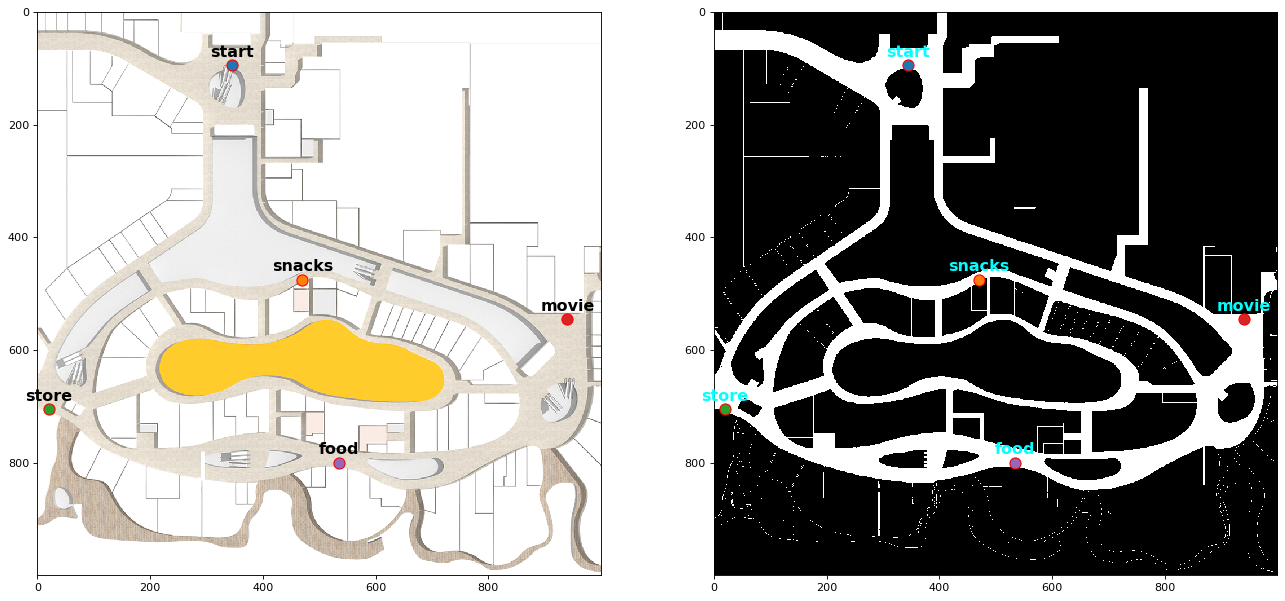
\includegraphics[width=12cm]{map.png}
	\caption{Original and grayscaled map of the Vivocity level 2}
	\label{fig1}
\end{figure} 

\subsection{Implement of A* algorithm}
\hspace{1.0em}

\begin{algorithm}[H]\footnotesize
	\SetAlgoLined
	\KwIn{start point $s_{start}$, goal point $s_{end}$}
	\KwOut{planned path $path$}
	
	Initialize $Openset$, $Closeset$, $g\_cost$ and $parent\_node$\;
	\While{$Openset$ is not empty}{
		Pop one node $s_{current}$ from the head of $Openset$\;
		Add $s_{current}$ to $Closeset$\;
		\If{$s_{current}$ is the goal point $s_{end}$}{
			break\;
		}
		\For{each neighbor node $s_{n}$ of $s_{current}$}{
			Compute the new $g\_cost$: $g_{new} = g\_cost[s_{current}] + edgecost(s_{current}, s_{n})$\;
			\If{$s_{n}$ not in $g\_cost$}{
				Initialize $g\_cost$ for $s_{n}$: $g\_cost[s_n] = inf$\;
			}
			\If{$g_{new} < g\_cost[s_{n}]$}{
				Rechoose the parent node: $parent\_node[s_{n}] = s$\;
				Update the $g\_cost$ for $s_{n}$: $g\_cost[s_{n}] = g_{new}$\;
				Compute the $f$ value for $s_{n}$: $f(s_{n}) = g\_cost[s_{n}] + h(s_{n})$\;
				Push the node $s_{n}$ with its $f$ value into $Openset$\;
			}
		}
	}
	Retrieve the final path $path$ from $s_{end}$ according to the parrent node dictionary $parrent\_node$\;
	\caption{A* path planning algorithm}
	\label{alg:algorithm1} 
\end{algorithm}


The workflow of A* algorithm is given in Alg.~\ref{alg:algorithm1}. At the beginning (line 1), we initialize one priority queue $Openset$, which will store the node with the highest $f$ value on the top. For each node $s$, we compute its $f$ value by:

\begin{equation}
\begin{aligned}
f(s) = g(s) + h(s)
\label{eq1}
\end{aligned}
\end{equation}

where $g(s)$ is the path length between $s$ and the start point $s_{start}$, while $h(s)$ is a heuristic function that measures the distance from $s$ to the goal $s_{end}$. In the initialization step, we push $s_{start}$ with its $f$ value $f(s_{start}) = h(s_{start})$ into the $Openset$. An empty $Closeset$ is also initialized to save the nodes that have been visited. One dictionary $g\_cost$ is used to store the $g$ value for each node, while $parent\_node$ dict records the parent of each node. We assume the node has a infinite $g$ value if there's no found path from $s_{start}$ to it, so we initialize $g\_cost[s_{end}] = inf$.   

For each current node $s_{current}$, we expand in 8 directions and compute the new $g$ value for each neighbor node $s_{n}$ (line 9). $edgecost(s_{current}, s_{n})$ is measured by the Euclidean distance between the two nodes, and it is set to be inifinite if there's an obstacle. Therefore, collision is checked according to the given footprint radius and map resolution in our algorithm. Then, if the new cost $g_{new}$ is less than its original value (a better path is found for this node), we update $g$ value and rechoose the parent node for it (line 14, 15). After that, the node $s_{n}$ with its computed $f$ value is pushed into the priority queue $Openset$ for future expansion (line 16, 17). 

The algorithm ends if the $Openset$ is empty (means no more nodes can be expanded and fail to find the path) or we finally expand to the goal point (line 5,6,7). If there exists one way from the start to destination, A* algorithm can always achieve the former case with a shortest path. The length of the optimal path can be got from the dict $g\_cost$ (i.e. $g\_cost[s_{end}]$), and all visited nodes are saved in $Closeset$. To evaluate our algorithm, we also record the searching time for further comparison. 

We first determine the heuristic function as the Euclidean distance between $s_{current}$ and $s_{end}$. For each key location on the map, we plot the planned paths from it to all other key locations with different color (Fig.~\ref{fig2}). Tab.~\ref{tab1} records the shortest distances between each pair of locations, and Tab.~\ref{tab2} \& \ref{tab3} saves the number of visited cells and running time. 

\begin{figure}[H]
	\centering
	\begin{minipage}[t]{0.32\textwidth}
		\centering
		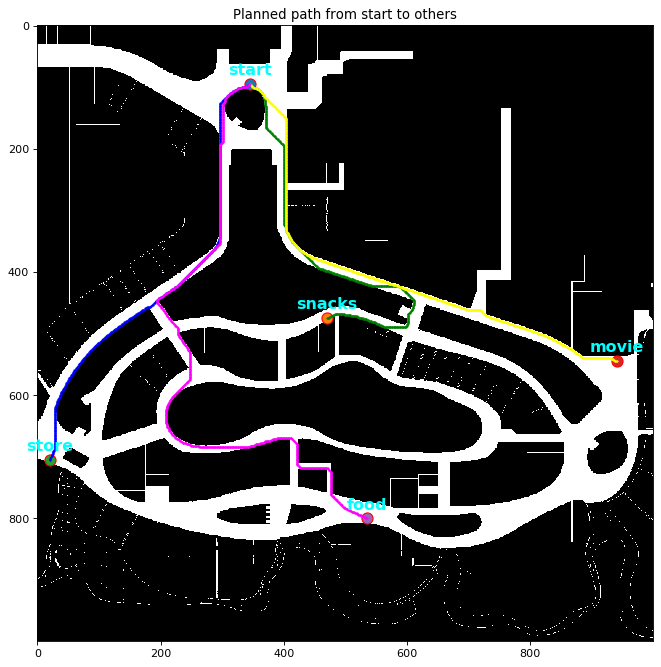
\includegraphics[width=4.5cm]{start_to_others.png}
		\subcaption{From "start" to other key locations}
		\label{fig2a}
	\end{minipage}
	\begin{minipage}[t]{0.32\textwidth}
		\centering
		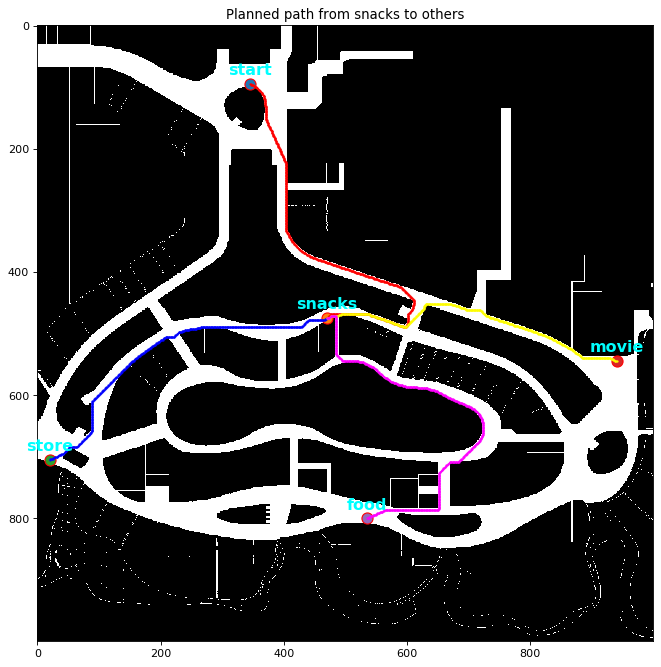
\includegraphics[width=4.5cm]{snacks_to_others.png}
		\subcaption{From "snacks" to other key locations}
		\label{fig2b}
	\end{minipage}
	\begin{minipage}[t]{0.32\textwidth}
		\centering
		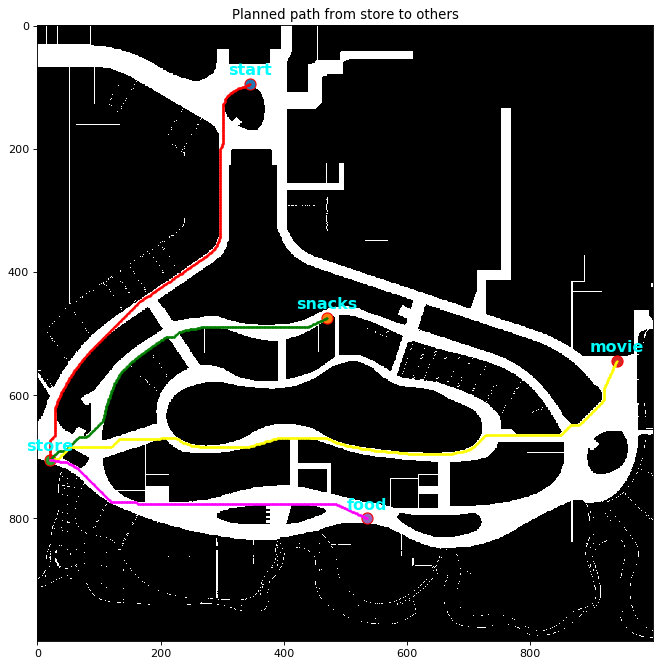
\includegraphics[width=4.5cm]{store_to_others.png}
		\subcaption{From "store" to other key locations}
		\label{fig2c}
	\end{minipage}
	\begin{minipage}[t]{0.45\textwidth}
		\centering
		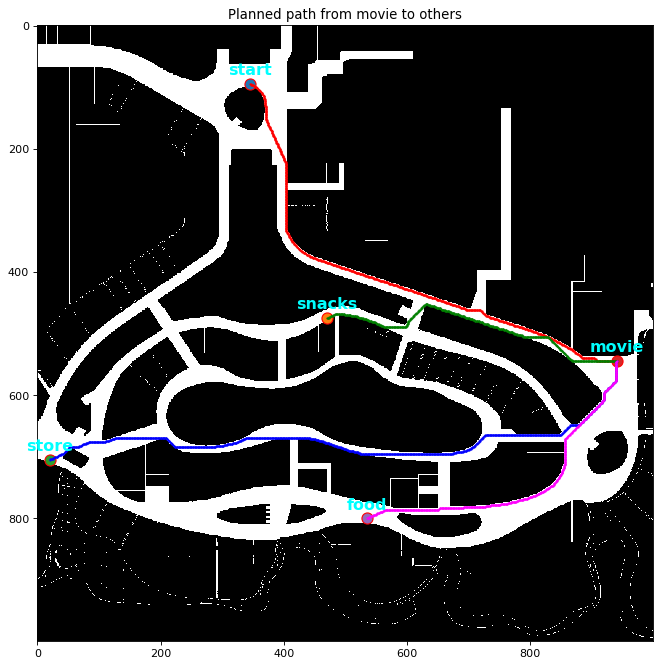
\includegraphics[width=4.5cm]{movie_to_others.png}
		\subcaption{From "movie" to other key locations}
		\label{fig2d}
	\end{minipage}
	\begin{minipage}[t]{0.45\textwidth}
		\centering
		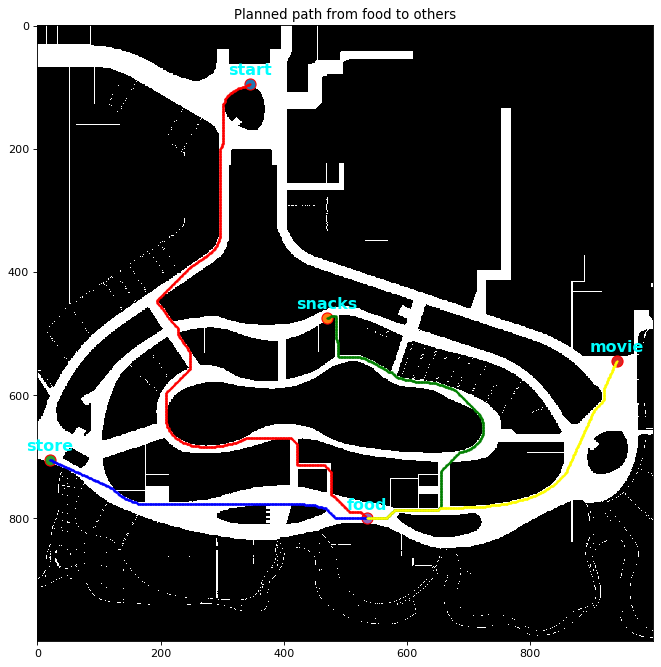
\includegraphics[width=4.5cm]{food_to_others.png}
		\subcaption{From "food" to other key locations}
		\label{fig2e}
	\end{minipage}
	\caption{Path planning using A* algorithm with Euclidean heuristic function}
	\label{fig2}
\end{figure} 


\begin{table}[H]
	\centering
	\begin{minipage}[c]{0.8\textwidth}
		\centering
		\caption{Path length between key locations (m)}
		\begin{tabular}{|c|c|c|c|c|c|}
			\hline
			\diagbox{To}{From} &start &snacks &store &movie &food \\
			\hline
			start &0.00 &142.49 &155.13 &178.89 &223.32 \\
			\hline
			snacks &142.49 &0.00 &114.79 &107.51 &133.43 \\
			\hline
			store &155.13 &114.79 &0.00 &209.42 &110.87 \\
			\hline
			movie &178.89 &107.51 &209.42 &0.00 &113.72 \\
			\hline
			food &223.32 &133.43 &110.87 &113.72 &0.00 \\
			\hline
		\end{tabular}
		\label{tab1}
	\end{minipage}
\end{table}

\begin{table}[H]
	\centering
	\begin{minipage}[c]{0.49\textwidth}
		\setlength{\tabcolsep}{0.5mm}
		\centering
		\caption{Number of visited cells for each pair}
		\begin{tabular}{|c|c|c|c|c|c|}
			\hline
			\diagbox{To}{From} &start &snacks &store &movie &food \\
			\hline
			start &0 &62604 &48950 &49582 &144731 \\
			\hline
			snacks &36173 &0 &25162 &13943 &43622 \\
			\hline
			store &57455 &38675 &0 &89265 &18468 \\
			\hline
			movie &42199 &14406 &52701 &0 &43275 \\
			\hline
			food &106389 &56255 &28002 &43050 &0 \\
			\hline
		\end{tabular}
		\label{tab2}
	\end{minipage}
	\begin{minipage}[c]{0.49\textwidth}
		\setlength{\tabcolsep}{0.5mm}
		\centering
		\caption{Running time for each pair (ms)}
		\begin{tabular}{|c|c|c|c|c|c|}
			\hline
			\diagbox{To}{From} &start &snacks &store &movie &food \\
			\hline
			start &0.00 &856.13 &440.20 &919.54 &606.72 \\
			\hline
			snacks &891.98 &0.00 &205.61 &777.32 &653.36 \\
			\hline
			store &670.79 &876.67 &0.00 &100.90 &243.30 \\
			\hline
			movie &31.48 &719.87 &949.57 &0.00 &132.90 \\
			\hline
			food &538.93 &747.51 &527.95 &404.79 &0.00 \\
			\hline
		\end{tabular}
		\label{tab3}
	\end{minipage}	
\end{table}

\subsection{Comparison of algorithm performance with different heuristic function}
\hspace{1.0em}

We find if the start and goal position are switched, the length of path found by A* algorithm is the same, whereas the path is not definitely the same (see the path from "start" to "snacks" in Fig.~\ref{fig2a} and \ref{fig2b}). This is due to the expansion process is not definite, so the number of visited cells as well as the algorithm's running time also changes. To test the performance of A* algorithm with different types of heuristic function, we change the metric to "Manhatan". Also, we degenerate the A* algorithm to Dijkstra's algorithm by setting $h(s)=0$. We take from "start" to others as an example (all other results are saved in the .ipynb file), and the results are shown in Fig.~\ref{fig3} and Tab.~\ref{tab4}. We can see all three algorithms find the optimal path, but Dijkstra's algorithm expands much more nodes and cost much longer time than the other two algorithms, which is because no heuristic function exists to guide it search towards the goal position. Of course, if we only consider the heuristic distance and ignore the $g$ value, A* algorithm will degenerate to Greedy Best First Search algorithm. In that case, the agent can expand quickly towards the goal and find the feasible path, but the path will be far from optimal.  

\begin{figure}[H]
	\centering
	\begin{minipage}[t]{0.49\textwidth}
		\centering
		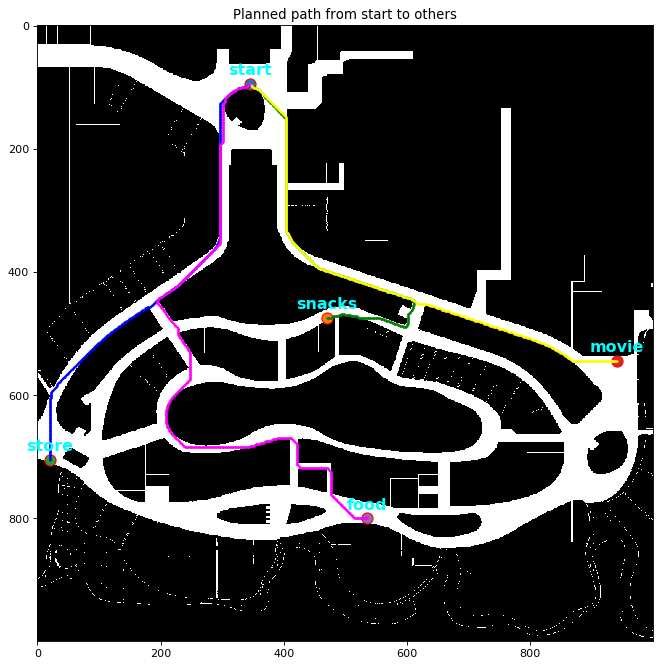
\includegraphics[width=5cm]{start_to_others_manhattan.png}
		\subcaption{A* (Manhattan heuristic function)}
		\label{fig3a}
	\end{minipage}
	\begin{minipage}[t]{0.49\textwidth}
		\centering
		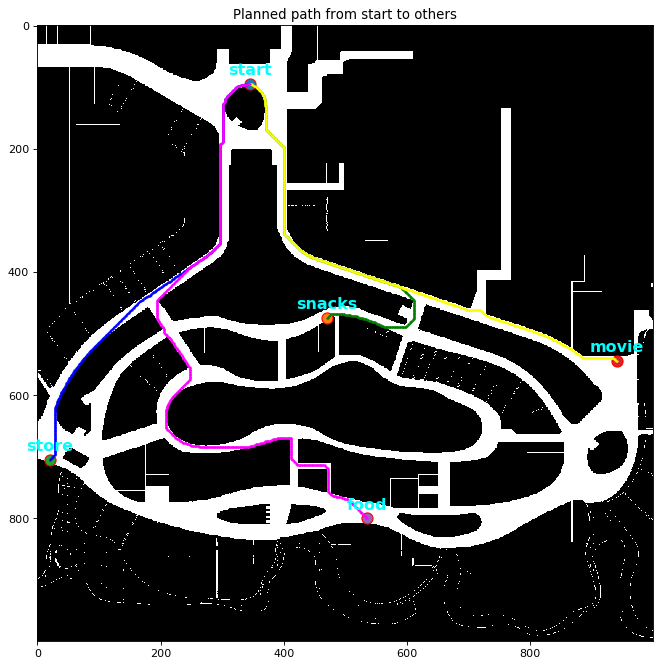
\includegraphics[width=5cm]{start_to_others_Dijkstra.png}
		\subcaption{Dijkstra's algorithm (without heuristic function)}
		\label{fig3b}
	\end{minipage}
	\caption{Performance of algorithm with different heuristic function (from "start" to "snacks")}
	\label{fig3}
\end{figure}

\begin{table}[H]
	\centering
	\begin{minipage}[c]{0.8\textwidth}
		\centering
		\caption{Performance of algorithm with different heuristic functions}
		\begin{tabular}{|c|c|c|c|c|c|}
			\hline
			Algorithm type &Metrics  &snacks &store &movie &food \\
			\hline
			&Path length (m) &142.49 &155.13 &178.89 &223.32 \\
			A* (Euclidean)&Visited cells &62604 &48950 &49582 &144731\\
			& Search time (ms) &856.13 &440.20 &919.54 &606.72 \\ 
			\hline
			&Path length (m) &142.49 &155.13 &178.90 &223.32 \\
			A* (Manhattan)&Visited cells &74603 &3304 &2801 &128348\\
			& Search time (ms) &620.63 &367.57 &63.91 &669.03 \\ 
			\hline
			&Path length (m) &142.49 &155.13 &178.89 &223.32 \\
			Dijkstra's&Visited cells &725364 &908754 &1309916 &2322154\\
			& Search time (ms) &4914.73 &5521.74 &10592.66 &21346.07 \\ 
			\hline
		\end{tabular}
		\label{tab4}
	\end{minipage}
\end{table}

We also find the Manhattan heuristic function can almost find the optimal path with less time and visited nodes than using Euclidean distance. However, using heuristic function with Manhattan metrics cannot always find the shortest path, since A* algorithm ensures optimality only when $h(s) \leq h^{*}(s)$, where $h^{*}(s)$ represents the real distance from node $s$ to goal position $s_{end}$ (easy to certify $h(s) > h^{*}(s)$ when using Manhattan distance). 



\subsection{Possible improvement methods}
\hspace{1.0em}

Actually, if we determine our expanding rule as 8-neighbor search, we can compute real distance $h^{*}$ in closed form (also known as Diagonal heuristic function):

\begin{equation}
\begin{aligned}
h(s) = (\left | x_{f}-x_{s} \right | + \left | y_{f}-y_{s} \right | + (\sqrt{2}-2)min\{\left | x_{f}-x_{s} \right |, \left | y_{f}-y_{s} \right |\})
\label{eq2}
\end{aligned}
\end{equation}

Another technique to reduce the visited nodes is to introduce a tie-breaker, which can break the symmetry of expanding directions. The modified heuristic function becomes:

\begin{equation}
h(s) := h(s)\cdot(1 + p)
\label{eq3}
\end{equation}

where $p$ is relevant to the map scale and often set as an extremely small number (0.0001 here). The algorithm performance is shown in Fig.~\ref{fig4}. We find the number of visited cells is reduced in two cases, and the search time is much less than that using Euclidean distance without tie-breaker.  


\begin{figure}[H]
	\begin{minipage}{.4\linewidth}
		\centering
		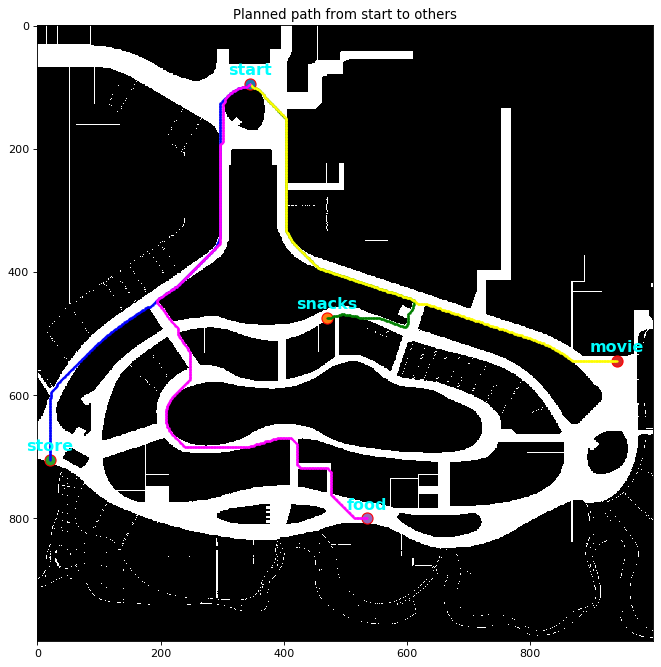
\includegraphics[width=5cm]{start_to_others_diagonal.png}
	\end{minipage}
	\begin{minipage}{.6\linewidth}
		\centering
		\begin{tabular}{|c|c|c|c|c|}
			\hline
			Metrics  &snacks &store &movie &food \\
			\hline
			Path length (m) &142.49 &155.13 &178.89 &223.32 \\
			Visited cells &76363 &35310 &47580 &154767\\
			Search time (ms) &185.549 &31.322 &292.285 &483.445 \\ 
			\hline
		\end{tabular}
	\end{minipage}
	\caption{Performance of A* algorithm after improvements}
	\label{fig4}
\end{figure}


\section{Task 3: The “Travelling Shopper” Problem}
\hspace{1.0em}

Given Tab.~\ref{tab1}, we are required to compute the optimal route to visit all stores and come back to the start location, which is also known as "Travelling Shopper Problem". The simplest way is to enumerate all possible routes and compare their total distance. The time complexity is $O(n!)$ and it can solve the problem quickly in our case since there are only 5 key locations. However, it will become extremely slow when more locations are added.

Another common method is model it as a dynamic programming problem. We define $d(i, V')$ as the lowest cost when the shopper reaches node $i$ and have been to all the nodes in set $V'$. We mark the start point as '0', so the initial condition becomes:


\begin{equation}
\begin{aligned}
d(0,\{0\}) = 0
\label{eq4}
\end{aligned}
\end{equation}

When we decide to arrive location 'i' with the lowest cost, we need to compute according to the distance matrix in Tab.~\ref{tab1} and the current state. Then we derive the transition equation:

\begin{equation}
\begin{aligned}
d(i, V'+\{i\}) = \min_{k \in V'}\{d(k, V') + c_{ki}\}
\label{eq5}
\end{aligned}
\end{equation}

After constructing the dynamic programming array, the total distance after coming back to the start point '0' can be obtained by:

\begin{equation}
\begin{aligned}
d\_total = \min_{i \in S} \{d(i, S) + c_{i0}\}
\label{eq6}
\end{aligned}
\end{equation}

where $S$ is the set including all locations (i.e. the shopper man has been to all locations). In our implementation, the set $V'$ has $2^{5}$ possible values and that for $i$ (the current location) is 5, so we construct the dynamic programming array in a shape of $[2^{5}, 5]$. One technique is to use a binary data to represent the set $V'$, which can facilitate the programming (for example, '11011' represent the set \{0,1,3,4\}). After filling the array according the initial condition in Eq.~\ref{eq4} and transition rule in Eq.~\ref{eq5}, we can directly get the total length by Eq.~\ref{eq6} and also easily obtain the route by retrieving the path from end to start.

We compare the violent enumeration and dynamic programming method by the total length, the whole route and time cost. As is shown in Fig.~\ref{fig5}, the total length computed and optimal route obtained are both the same (the route order is just inversed). Surprisingly, in this case the violent enumeration method cost less time than dynamic programming method, since there are only 5 locations here. Actually, the time complexity for the DP method is $O(2^{n}n^{2})$, so when $n$ becomes larger, the DP method can work much more efficiently than the simple enumeration method. We plot the obtained optimal route in Fig.~\ref{fig6}. 

 
\begin{figure}[H]
		\centering
		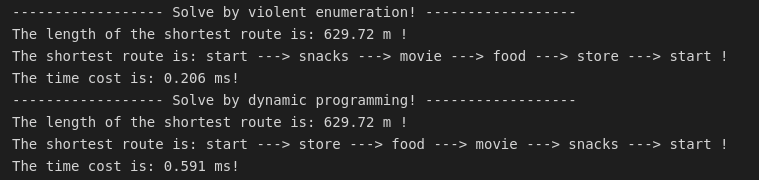
\includegraphics[width=8cm]{compare.png}
	\caption{Comparison between the two methods}
	\label{fig5}
\end{figure}

\begin{figure}[H]
	\centering
	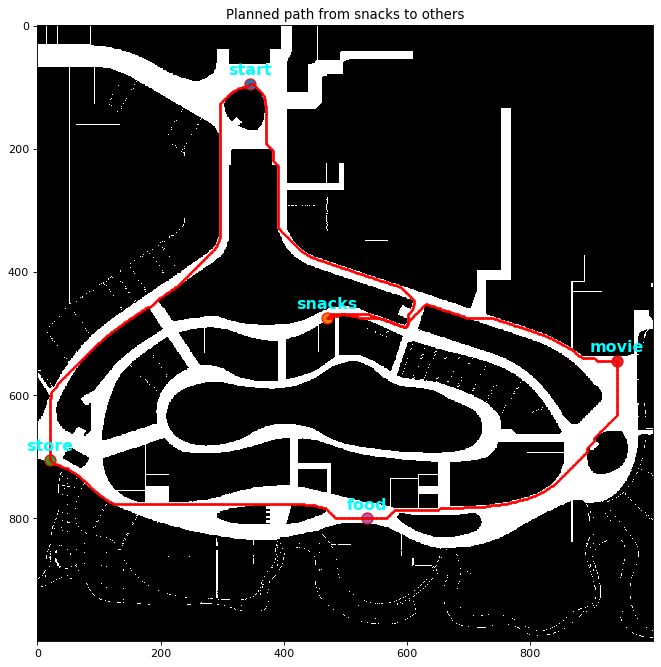
\includegraphics[width=5cm]{optimal_route.png}
	\caption{The optimal route obtained by DP method}
	\label{fig6}
\end{figure}

\newpage

%\begin{appendices}
%	\section{xxx}
%	
%	\section{xxx}
%	
%\end{appendices}





	
\end{document}








